\documentclass[11pt]{article}
\usepackage{multirow}
\usepackage{hyperref}
\usepackage[margin=1in, top=1.5in]{geometry} 
\usepackage{titling} 
\usepackage{fancyhdr}
\usepackage{cancel}
\usepackage{amsmath}
\usepackage{graphicx}
\usepackage{ragged2e}
\usepackage{calc}
\usepackage{here}
\usepackage{siunitx}




\setlength{\droptitle}{-3cm} 
\pagestyle{fancy}
\fancyhf{} 
\lhead{EN.566: Introduction to Computational Materials Modeling 2023 - HW2}
\rhead{Amitabh Roy}

\begin{document}

\section{Problem Description}
The objective of the HW2 is to solve the problem of radioactive decay of C-14 isotope and also to predict the trajectory of the gold ball. The radioactivity and the golf trajectory problem can be solved using the Euler's method and finally write a python code for doing the calculations.  Mathematical relations for section can be found below:

\section{Solution to Carbon Dating Problem}

In this problem we have to derive a relation between half-life time $t_{1/2}$ and decay constant $\tau$,  plot the number of particles left vs time over the duration of 20,000 years and with different step size (10, 100, 1000 years)

\subsection{Derive analytically the relation between half-life time  and decay constant as defined in class.}
let, N = Number of nuclie at any given time 't', t = time, $\Delta$N = Number of nuclie undergoing decay at time 't'

So, $\Delta$N $\propto $ N*$\Delta$t

$\Delta$N = -$\tau$ N*$\Delta$t {Where, $\tau$ is the decay constant}

On rearranging,
$\frac{\Delta N}{N}$ = -$\tau$*$\Delta$t

Integrating for initial nuclie = $N_{o}$ and final nuclie = $\frac{N_{o}}{2}$ \& stating time  = 0 , final time = $t_{1/2}$)

$\int_{N_{o}}^{\frac{N_{o}}{2}}\frac{\Delta N}{N} = \int_{0}^{t_{1/2}}-\tau*\Delta t$

$\log\frac{N_{o}}{2} - \log N_{o} = -\tau*t_{1/2}$

$\log\frac{\cancel{N_{o}}}{2*\cancel{N_{o}}} = -\tau*t_{1/2}$

$\log\frac{1}{2} = -\tau*t_{1/2}$. 

Therefore, $\tau = -\frac{\log\ 0.5}{t_{1/2}}$.
In the problem it is given that the half life is 5700 years.

Value of $\tau = -\frac{\log\ 0.5}{5700}$

$\tau$ = 8223.36\, \text{years}\textsuperscript{-1}


\subsection{Python code to plot the rate of the radioactive decay vs time}
\begin{raggedright}
\begin{justify}
\textbf{Approach:}\\
To have a better interface with the command line the argparse library is selected. Once the setting up is done some variables like $\tau$, $N_{o}$ and $t_{1/2}$ are defined. Then empty lists like time, number\_particle\_at\_t and rate are also defined to store the value that we will be calculating in the for loop and then using the 'del'. And once done with the plotting of one set the elements of the list are deleted to store the values for different step width.
\end{justify}
\end{raggedright}

\begin{raggedright}
\begin{justify}
\textbf{Algorithm:}\\
To better optimize the code a nested 'for' loop is selected. First loop is to cycle through the list of the step width with a prerequisite step which deletes all the elements of the lists and the $2^{nd}$ loop is for calculating ans storing the values associated for the number of particle at time = t and also time 't'.\\
At t= 0, number\_particle\_at\_t = $N_{o}$ .\\
And for other steps - \\
\textbf{\( \text{number\_particle\_at\_t}[i]=\text{number\_particle\_at\_t}[i-1] - \frac{1}{\tau} \cdot \text{number\_particle\_at\_t}[i-1] \cdot \text{step\_width}\)} \\
To finally find the value of the rate following formula is used\\
\textbf{Rate[i] = (number\_particle\_at\_t[i-1] - number\_particle\_at\_t[i])/\text{step\_width}}\\
Refer \hyperref[fig:Rate of radioactive decay for step width = 10, 100]{Figure 1} for the Rate vs time plot
\end{justify}
\end{raggedright}

\begin{figure}[b]
    \centering
    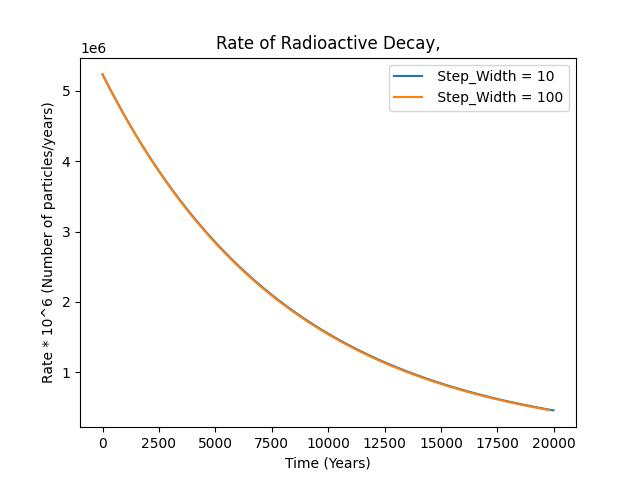
\includegraphics[width=\textwidth, height=\textheight, keepaspectratio]{Carbon_plot_10_100.jpeg}
    \caption{Rate of radioactive decay for step width = 10, 100}
    \label{fig:Rate of radioactive decay for step width = 10, 100}
\end{figure}

\subsection{To consider a step width of 1000 years and then find the percentage deviation from the exact result after 2 half-lives}

Firstly a new plot is made with 1000 years as a step width(Figure 2).
To find the value of the rate at 2 times of half life, a library called \textbf{'numpy'} is used as following: rate\_interp = numpy.interp(2*$t_{1/2}$, value of x axis, value of y axis)
Also, in the problem there has be a comparison made, like if we consider the 2nd order of the taylor expansion, will there be any improvement in the prediction?
Taylor series is as follows,
$N(t+\Delta t) = N(t) - \frac{\tau \Delta t}{2} N(t) + \frac{\tau^2 (\Delta t)^2}{2}$\\
Following is the output from the python code (Refer \hyperref[fig:Rate of radioactive decay for step width = 10, 100, 1000]{Figure 2} for the overview plot):
\begin{enumerate}
    \item Rate at 11400 years = 1306582.89 ;for step width = 10.
    \item Rate at 11400 years = 1296619.98 ;for step width = 100.
    \item Rate at 11400 years = 1195355.27 ;for step width = 1000.
    \item Rate at 11400 years = 1234940.25 ;for step width = 1000 considering the 2nd order.
\end{enumerate}
Conclusion: When comparing the step width of 1000 years, it has percentage of deviation as following (Refer \hyperref[fig:Rate of radioactive decay for step width = 1000, with 2nd order term]{Figure 3} for the comparison plot):
\begin{raggedright}
\begin{justify}
Without 2nd order = $\frac{\left|1195355.27 - 1306582.89\right|}{1306582.89} \times 100 = 8\%$\\
With 2nd order = $\frac{\left|1234940.25 - 1306582.89\right|}{1306582.89} \times 100 = 5\% $\\
So, it is clear that deviation from the exact result can be reduced if we include second-order term. But the key is to keep the step width as small as possible.
\end{justify}
\end{raggedright}


\begin{figure}[b]
    \centering
    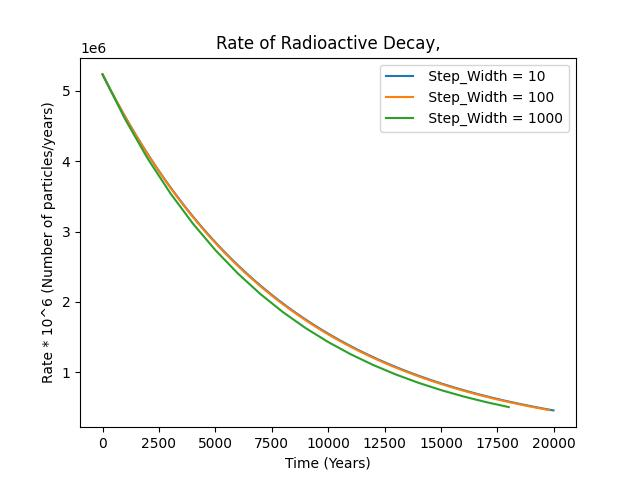
\includegraphics[width=\textwidth, height=\textheight, keepaspectratio]{Carbon_plot_10_100_1000.jpeg}
    \caption{Rate of radioactive decay for step width = 10, 100, 1000}
    \label{fig:Rate of radioactive decay for step width = 10, 100, 1000}
\end{figure}

\begin{figure}[b]
    \centering
    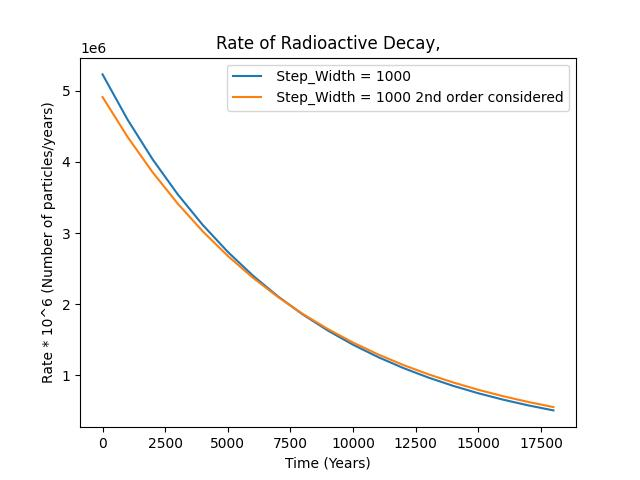
\includegraphics[width=\textwidth, height=\textheight, keepaspectratio]{Carbon_plot_1000_with 2nd order.jpeg}
    \caption{Rate of radioactive decay for step width = 1000, with 2nd order term}
    \label{fig:Rate of radioactive decay for step width = 1000, with 2nd order term}
\end{figure}


\section{Solution to Golf trajectory problem}
In this problem we have write a program to calculate the trajectory of a golf ball as a function of angle($\theta$). There are 4 cases, ideal, smooth ball with drag, dimpled ball with drag and dimpled ball with drag and a spin.
\subsection{Ideal trajectory}
\begin{raggedright}
let, 'x' coordinate of x-axis and 'y' be the coordinate of the y-axis; 'vx' and 'vy' be the velocity of the projectile along x-axis and y-axis respectively; 'g' be thw acceleration due to gravity which will act against the motion of the ball and m be the mass of the ball\\
Also for ideal condition,\\
$\frac{\text{dx}}{\text{dt}}$ = vx , \\
$\frac{\text{dx}}{\text{dt}}$ = vy , \\
$\frac{\text{dvx}}{\text{dt}}$ = 0 , \\
$\frac{\text{dvx}}{\text{dt}}$ = -g , \\
On solving the taylor series of the x(t+dt), vx(t+dt) , y(t+dt) , vy(t+dt)\\
We get,\\
x(t+dt) = x(t) + $\frac{\text{dx}}{\text{dt}}$ *dt = x(t) + vx *dt\\
vx(t+dt) = vx(t) + $\frac{\text{dvx}}{\text{dt}}$ *dt = vx(t)\\
y(t+dt) = y(t) + $\frac{\text{dy}}{\text{dt}}$ *dt = y(t) + vy *dt\\
vy(t+dt) = vy(t) + $\frac{\text{dvy}}{\text{dt}}$ *dt = vy(t) - g*dt\\

\end{raggedright}

\begin{raggedright}
\begin{justify}
Using these simplified equation, 'while' loop can be written\\
To start, lists like x\_trajectory, y\_trajectory, vx, vy are defined.At t=0 x\_trajectory and y\_trajectory will be equal to '0'. And vx, vy will be equal to the cos and sin component of the initial velocity i.e. 70 m/s. Here 'while' loop can be used and the exit condition will be when the value of y\_trajectory again becomes '0' or a value which is very close to zero. Same 'while' loop will be used in the remaining 3 conditions.
\end{justify}
\end{raggedright}

\begin{raggedright}
\begin{justify}
x\_trajectory[i+1] = x\_trajectory[i]+vx[i]*dt\\
vx[i+1] = vx[i]\\
y\_trajectory[i+1] = y\_trajectory[i]+vy[i]*dt \textit{(loop will run untill it is again zero)}\\
vy[i+1] = vy[i]-g*dt\\
Refer \hyperref[fig:ideal_trajectory]{Figure 4} for the comparison plot

\end{justify}
\end{raggedright}

\begin{figure}[b]
    \centering
    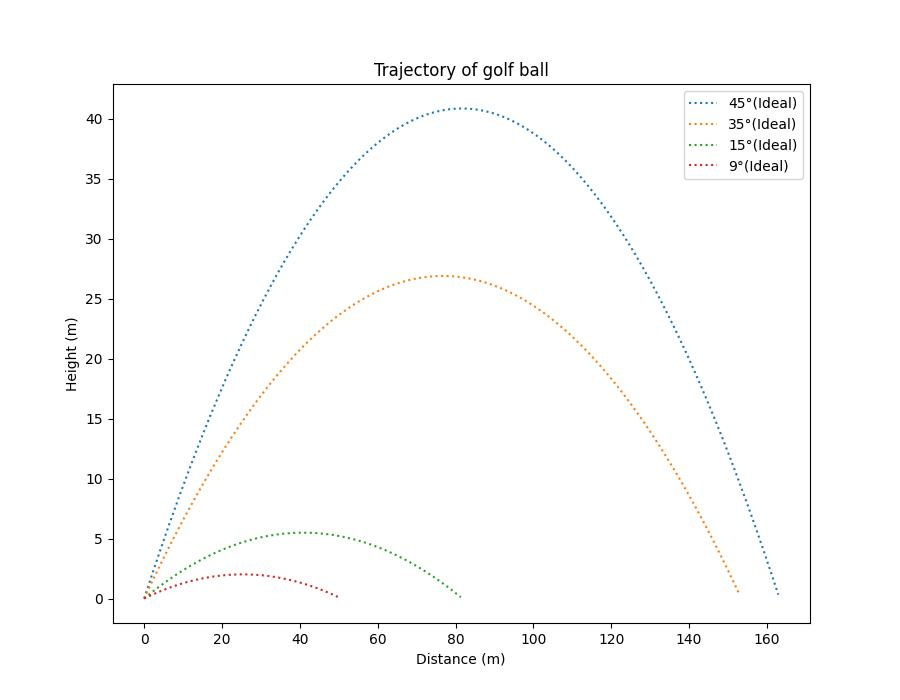
\includegraphics[width=\textwidth, height=\textheight, keepaspectratio]{Golf_Trajectory_Ideal.jpeg}
    \caption{Smooth Golf ball trajectory with external force acting on it $\theta$ = 45, 30, 15 and 9 degrees}
    \label{fig:ideal_trajectory}
\end{figure}

\subsection{Smooth ball with drag}

\(F_{\text{drag}} = -C \rho A v^2\), 
where \(\rho\) is the density of air (at sea level) \(= 1.29 \, \text{kg/m}^3\), \(A\) is the frontal area of the golf ball \(= 0.0014 \, \text{m}^2\), \(C\) is a coefficient \(= 0.5\), and \(v = \sqrt{v_x^2 + v_y^2}\).
\begin{raggedright}
\begin{justify}
x\_trajectory[i+1] = x\_trajectory[i]+vx[i]*dt\\
y\_trajectory[i+1] = y\_trajectory[i]+vy[i]*dt \textit{(loop will run until y\_trajectory is zero again)}\\
vx[i+1] = vx[i]-$\frac{-0.5*0.0014*1.29*\sqrt{vx^2+vy^2}*vx[i]}{m}*dt$\\
vy[i+1] = vy[i]-g*dt-$\frac{-0.5*0.0014*1.29*\sqrt{vx^2+vy^2}*vy[i]}{m}*dt$\\
Refer \hyperref[fig:Smooth_Fdrag_trajectory]{Figure 5} for the comparison plot
\end{justify}
\end{raggedright}


\begin{figure}[b]
    \centering
    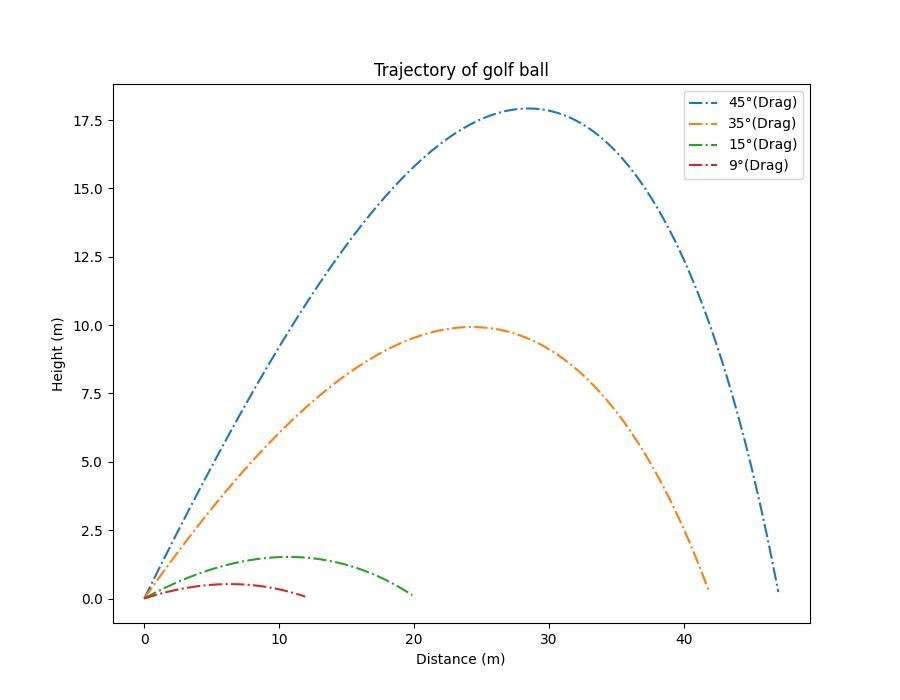
\includegraphics[width=\textwidth, height=\textheight, keepaspectratio]{Golf_Trajectory_Smooth_Drag.jpeg}
    \caption{Smooth Golf ball trajectory with drag force acting on it $\theta$ = 45, 30, 15 and 9 degrees}
    \label{fig:Smooth_Fdrag_trajectory}
\end{figure}

\subsection{Dimpled ball with drag}

\( F_{\text{drag}} = -C \cdot \rho \cdot A \cdot v^2 \), where \( C = \begin{cases} 0.5 & \text{for } v \leq 14 \, \text{m/s} \\ \frac{7}{v} & \text{for } v > 14 \, \text{m/s} \end{cases} \), \( \rho = 1.29 \, \text{kg/m}^3 \), \( A = 0.0014 \, \text{m}^2 \), and \( v = \sqrt{v_x^2 + v_y^2} \).
\begin{raggedright}
\begin{justify}
x\_trajectory[i+1] = x\_trajectory[i]+vx[i]*dt\\
y\_trajectory[i+1] = y\_trajectory[i]+vy[i]*dt \textit{(loop will run until y\_trajectory is zero again)}\\
vx[i+1] = vx[i]-$\frac{-C*0.0014*1.29*\sqrt{vx^2+vy^2}*vx[i]}{m}*dt$\\
vy[i+1] = vy[i]-g*dt-$\frac{-C*0.0014*1.29*\sqrt{vx^2+vy^2}*vy[i]}{m}*dt$\\
Refer \hyperref[fig:Dimpled_Fdrag_trajectory]{Figure 6} for the comparison plot
\end{justify}
\end{raggedright}

\begin{figure}[b]
    \centering
    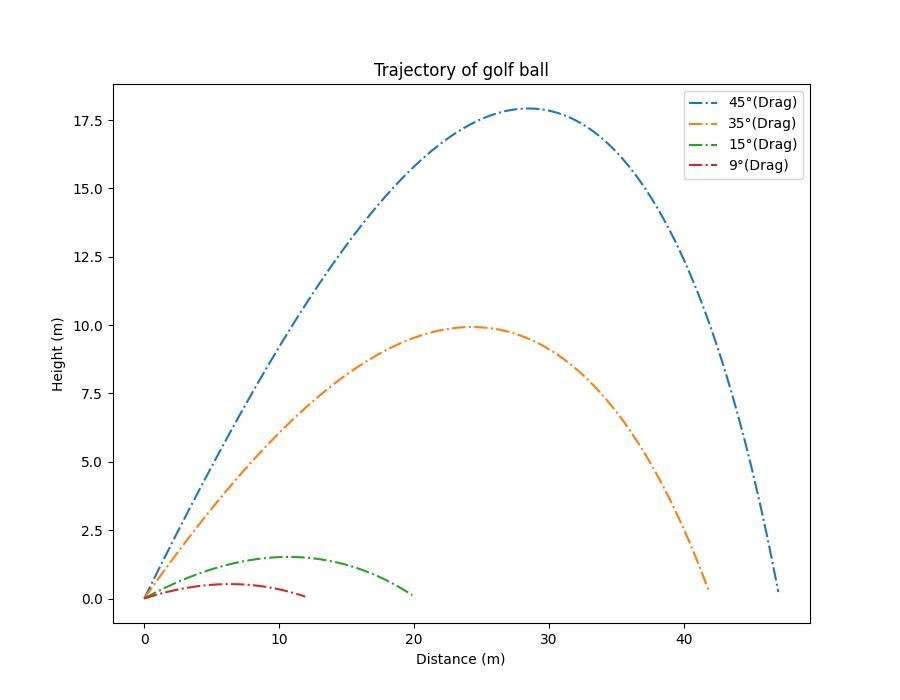
\includegraphics[width=\textwidth, height=\textheight, keepaspectratio]{Golf_Trajectory_Smooth_Drag.jpeg}
    \caption{Dimpled Golf ball trajectory with drag force acting on it $\theta$ = 45, 30, 15 and 9 degrees}
    \label{fig:Dimpled_Fdrag_trajectory}
\end{figure}

\subsection{Dimpled ball with drag and spin}

As, \(F_{\text{drag}} = -C\rho Av^2\), where \(\rho\) is the density of air (at sea level) \(= 1.29 \, \text{kg/m}^3\), \(A\) is the frontal area of the golf ball \(= 0.0014 \, \text{m}^2\), and \(C\) is a coefficient \(= 0.5\), \(v = \sqrt{v_x^2 + v_y^2}\).
And, \(F_{\text{Magnus}} = S_0 \cdot (\omega \times v)\) with a backspin of \(S_0 \cdot \frac{\omega}{m} = 0.25 \, \text{s}^{-1}\) for a typical case.

\begin{raggedright}
\begin{justify}
x\_trajectory[i+1] = x\_trajectory[i]+vx[i]*dt\\
y\_trajectory[i+1] = y\_trajectory[i]+vy[i]*dt \textit{(loop will run until y\_trajectory is zero again)}\\
vx[i+1] = vx[i]-$\frac{-C*0.0014*1.29*\sqrt{vx^2+vy^2}*vx[i]}{m}*dt - \frac{S_0 * \omega}{m}*vy[i]*dt$\\
vy[i+1] = vy[i]-g*dt-$\frac{-C*0.0014*1.29*\sqrt{vx^2+vy^2}*vy[i]}{m}*dt + \frac{S_0 * \omega}{m}*vx[i]*dt$\\
Refer \hyperref[fig:Spin_Dimpled_Fdrag_trajectory]{Figure 7} for the comparison plot\\
Refer \hyperref[fig:trajectory]{Figure 8} for comparing all the 4 scenarios together
\end{justify}
\end{raggedright}
\begin{figure}[b]
    \centering
    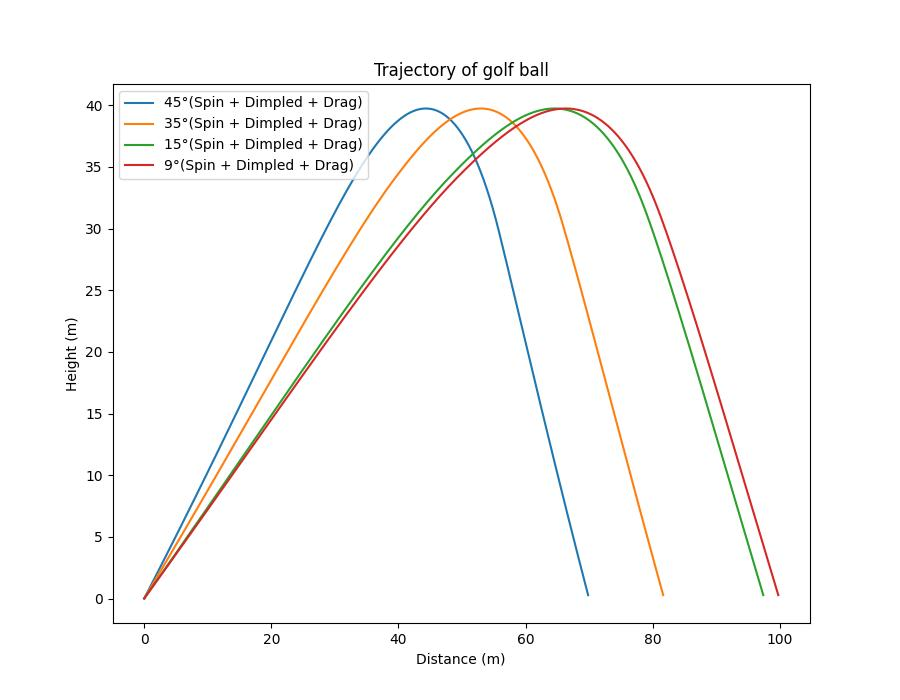
\includegraphics[width=\textwidth, height=\textheight, keepaspectratio]{Golf_Trajectory_Spin_Dimpled_drag.jpeg}
    \caption{Dimpled Golf ball trajectory with spin and drag force acting on it $\theta$ = 45, 30, 15 and 9 degrees}
    \label{fig:Spin_Dimpled_Fdrag_trajectory}
\end{figure}

\begin{figure}[b]
    \centering
    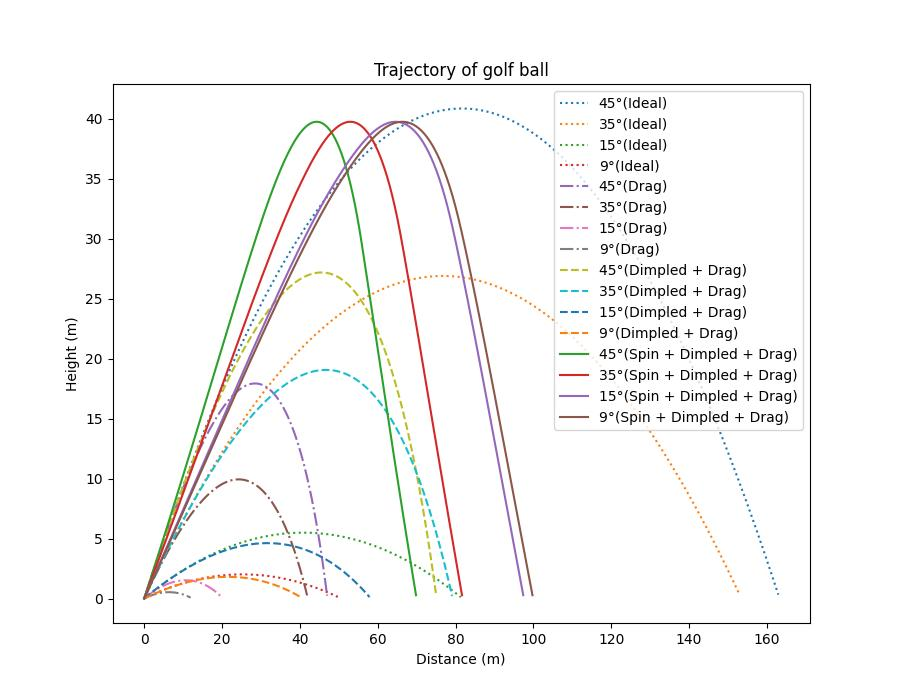
\includegraphics[width=\textwidth, height=\textheight, keepaspectratio]{Golf_Trajectory.jpeg}
    \caption{Golf ball trajectory - Comparision $\theta$ = 45, 30, 15 and 9 degrees}
    \label{fig:trajectory}
\end{figure}
\section{Contributions}
\begin{enumerate}
    \item I would like to thanks the Professor Corey Oses, Teaching Assistant Kumar Miskin , Alison and Jelly. It was their  teaching and/or initial round of discussion which gave me the framework to think on.
\end{enumerate}

  
\end{document}